\documentclass[]{article}

\usepackage{graphicx,type1cm,eso-pic,color}
\usepackage[spanish]{babel} %%%% for


\makeatletter
          \AddToShipoutPicture{
            \setlength{\@tempdimb}{.95\paperwidth}
            \setlength{\@tempdimc}{.5\paperheight}
            \setlength{\unitlength}{1pt}
            \put(\strip@pt\@tempdimb,\strip@pt\@tempdimc){
        \makebox(0,0){\rotatebox{-90}{\textcolor[gray]{0.90}
        {\fontsize{.65cm}{.5cm}\selectfont{\rm Dae-Jin Lee}}}}
            }
        }
          \AddToShipoutPicture{
            \setlength{\@tempdimb}{.50\paperwidth}
            \setlength{\@tempdimc}{.95\paperheight}
            \setlength{\unitlength}{1pt}
            \put(\strip@pt\@tempdimb,\strip@pt\@tempdimc){
        \makebox(0,0){\rotatebox{0}{\textcolor[gray]{0.90}
        {\fontsize{.5cm}{.5cm}\selectfont{\rm Curso de Estad\'istica b\'asica para Data Scientist  - @datahack}}}}
            }
        }
\makeatother

\def\tightlist{}

\usepackage{lmodern}
\usepackage{amssymb,amsmath}
\usepackage{ifxetex,ifluatex}
\usepackage{fixltx2e} % provides \textsubscript
\ifnum 0\ifxetex 1\fi\ifluatex 1\fi=0 % if pdftex
  \usepackage[T1]{fontenc}
  \usepackage[utf8]{inputenc}
\else % if luatex or xelatex
  \ifxetex
    \usepackage{mathspec}
    \usepackage{xltxtra,xunicode}
  \else
    \usepackage{fontspec}
  \fi
  \defaultfontfeatures{Mapping=tex-text,Scale=MatchLowercase}
  \newcommand{\euro}{???}
\fi
% use upquote if available, for straight quotes in verbatim environments
\IfFileExists{upquote.sty}{\usepackage{upquote}}{}
% use microtype if available
\IfFileExists{microtype.sty}{%
\usepackage{microtype}
\UseMicrotypeSet[protrusion]{basicmath} % disable protrusion for tt fonts
}{}
\usepackage{color}
\usepackage{fancyvrb}
\newcommand{\VerbBar}{|}
\newcommand{\VERB}{\Verb[commandchars=\\\{\}]}
\DefineVerbatimEnvironment{Highlighting}{Verbatim}{commandchars=\\\{\}}
% Add ',fontsize=\small' for more characters per line
\usepackage{framed}
\definecolor{shadecolor}{RGB}{248,248,248}
\newenvironment{Shaded}{\begin{snugshade}}{\end{snugshade}}
\newcommand{\KeywordTok}[1]{\textcolor[rgb]{0.13,0.29,0.53}{\textbf{{#1}}}}
\newcommand{\DataTypeTok}[1]{\textcolor[rgb]{0.13,0.29,0.53}{{#1}}}
\newcommand{\DecValTok}[1]{\textcolor[rgb]{0.00,0.00,0.81}{{#1}}}
\newcommand{\BaseNTok}[1]{\textcolor[rgb]{0.00,0.00,0.81}{{#1}}}
\newcommand{\FloatTok}[1]{\textcolor[rgb]{0.00,0.00,0.81}{{#1}}}
\newcommand{\ConstantTok}[1]{\textcolor[rgb]{0.00,0.00,0.00}{{#1}}}
\newcommand{\CharTok}[1]{\textcolor[rgb]{0.31,0.60,0.02}{{#1}}}
\newcommand{\SpecialCharTok}[1]{\textcolor[rgb]{0.00,0.00,0.00}{{#1}}}
\newcommand{\StringTok}[1]{\textcolor[rgb]{0.31,0.60,0.02}{{#1}}}
\newcommand{\VerbatimStringTok}[1]{\textcolor[rgb]{0.31,0.60,0.02}{{#1}}}
\newcommand{\SpecialStringTok}[1]{\textcolor[rgb]{0.31,0.60,0.02}{{#1}}}
\newcommand{\ImportTok}[1]{{#1}}
\newcommand{\CommentTok}[1]{\textcolor[rgb]{0.56,0.35,0.01}{\textit{{#1}}}}
\newcommand{\DocumentationTok}[1]{\textcolor[rgb]{0.56,0.35,0.01}{\textbf{\textit{{#1}}}}}
\newcommand{\AnnotationTok}[1]{\textcolor[rgb]{0.56,0.35,0.01}{\textbf{\textit{{#1}}}}}
\newcommand{\CommentVarTok}[1]{\textcolor[rgb]{0.56,0.35,0.01}{\textbf{\textit{{#1}}}}}
\newcommand{\OtherTok}[1]{\textcolor[rgb]{0.56,0.35,0.01}{{#1}}}
\newcommand{\FunctionTok}[1]{\textcolor[rgb]{0.00,0.00,0.00}{{#1}}}
\newcommand{\VariableTok}[1]{\textcolor[rgb]{0.00,0.00,0.00}{{#1}}}
\newcommand{\ControlFlowTok}[1]{\textcolor[rgb]{0.13,0.29,0.53}{\textbf{{#1}}}}
\newcommand{\OperatorTok}[1]{\textcolor[rgb]{0.81,0.36,0.00}{\textbf{{#1}}}}
\newcommand{\BuiltInTok}[1]{{#1}}
\newcommand{\ExtensionTok}[1]{{#1}}
\newcommand{\PreprocessorTok}[1]{\textcolor[rgb]{0.56,0.35,0.01}{\textit{{#1}}}}
\newcommand{\AttributeTok}[1]{\textcolor[rgb]{0.77,0.63,0.00}{{#1}}}
\newcommand{\RegionMarkerTok}[1]{{#1}}
\newcommand{\InformationTok}[1]{\textcolor[rgb]{0.56,0.35,0.01}{\textbf{\textit{{#1}}}}}
\newcommand{\WarningTok}[1]{\textcolor[rgb]{0.56,0.35,0.01}{\textbf{\textit{{#1}}}}}
\newcommand{\AlertTok}[1]{\textcolor[rgb]{0.94,0.16,0.16}{{#1}}}
\newcommand{\ErrorTok}[1]{\textcolor[rgb]{0.64,0.00,0.00}{\textbf{{#1}}}}
\newcommand{\NormalTok}[1]{{#1}}
\usepackage{longtable,booktabs}
\usepackage{graphicx}
\makeatletter
\def\maxwidth{\ifdim\Gin@nat@width>\linewidth\linewidth\else\Gin@nat@width\fi}
\def\maxheight{\ifdim\Gin@nat@height>\textheight\textheight\else\Gin@nat@height\fi}
\makeatother
% Scale images if necessary, so that they will not overflow the page
% margins by default, and it is still possible to overwrite the defaults
% using explicit options in \includegraphics[width, height, ...]{}
\setkeys{Gin}{width=\maxwidth,height=\maxheight,keepaspectratio}
\ifxetex
  \usepackage[setpagesize=false, % page size defined by xetex
              unicode=false, % unicode breaks when used with xetex
              xetex]{hyperref}
\else
  \usepackage[unicode=true]{hyperref}
\fi
\hypersetup{breaklinks=true,
            bookmarks=true,
            pdfauthor={Dae-Jin Lee \textless{} lee.daejin@gmail.com \textgreater{}},
            pdftitle={Curso de Estadística básica para Data Scientists},
            colorlinks=true,
            citecolor=blue,
            urlcolor=blue,
            linkcolor=magenta,
            pdfborder={0 0 0}}
\urlstyle{same}  % don't use monospace font for urls
\setlength{\parindent}{0pt}
\setlength{\parskip}{6pt plus 2pt minus 1pt}
\setlength{\emergencystretch}{3em}  % prevent overfull lines
\setcounter{secnumdepth}{5}

\title{\textbf{Curso de Estadística básica para Data Scientists}}
\author{Dae-Jin Lee \textless{}
\href{mailto:lee.daejin@gmail.com}{\nolinkurl{lee.daejin@gmail.com}}
\textgreater{}}
\date{\textbf{TEMA 4. Variables Aleatorias y Probabilidad}}

\usepackage{amsfonts}
\usepackage{amsmath}
\usepackage{amssymb}
\usepackage{natbib}
%\usepackage[T1]{fontenc}
\usepackage{latexsym}
\usepackage{graphicx}
\usepackage{caption}
\usepackage{subcaption}
\usepackage{color}
\usepackage{algorithm2e}
%%
%     Definitions
%
\newcommand{\tri}{\bigtriangleup}
\newcommand{\Xp}{X^\prime}
\newcommand{\E}{\mbox{E}}
\newcommand{\Hh}{\mbox{H}}
\newcommand{\V}{\mbox{Var}}
\newcommand{\tr}{\mbox{tr}}
\newcommand{\CV}{\mbox{CV}}
\newcommand{\GCV}{\mbox{GCV}}
\newcommand{\AIC}{\mbox{AIC}}
\newcommand{\ph}{\phantom{0}}
\newcommand{\half}{\mbox{${1\over2}$}}
\newcommand{\bfzero}{\boldsymbol{0}}
\newcommand{\bfone}{\boldsymbol{1}}

\newcommand{\bfa}{\boldsymbol{a}}
\newcommand{\bfb}{\boldsymbol{b}}
\newcommand{\bfe}{\boldsymbol{e}}
\newcommand{\bff}{\boldsymbol{f}}
\newcommand{\bfg}{\boldsymbol{g}}
\newcommand{\bfs}{\boldsymbol{s}}
\newcommand{\bfu}{\boldsymbol{u}}
\newcommand{\bfx}{\boldsymbol{x}}
\newcommand{\bfy}{\boldsymbol{y}}
\newcommand{\bfz}{\boldsymbol{z}}

\newcommand{\bfA}{\boldsymbol{A}}
\newcommand{\bfB}{\boldsymbol{B}}
\newcommand{\bfC}{\boldsymbol{C}}
\newcommand{\bfD}{\boldsymbol{D}}
\newcommand{\bfF}{\boldsymbol{F}}
\newcommand{\bfG}{\boldsymbol{G}}
\newcommand{\bfH}{\boldsymbol{H}}
\newcommand{\bfI}{\boldsymbol{I}}
\newcommand{\bfM}{\boldsymbol{M}}
\newcommand{\bfP}{\boldsymbol{P}}
\newcommand{\bfQ}{\boldsymbol{Q}}
\newcommand{\bfR}{\boldsymbol{R}}
\newcommand{\bfS}{\boldsymbol{S}}
\newcommand{\bfT}{\boldsymbol{T}}
\newcommand{\bfU}{\boldsymbol{U}}
\newcommand{\bfV}{\boldsymbol{V}}
\newcommand{\bfW}{\boldsymbol{W}}
\newcommand{\bfX}{\boldsymbol{X}}
\newcommand{\bfY}{\boldsymbol{Y}}
\newcommand{\bfZ}{\boldsymbol{Z}}


\newcommand{\bfalpha}{\boldsymbol{\alpha}}
\newcommand{\bfbeta}{\boldsymbol{\beta}}
\newcommand{\bfepsilon}{\boldsymbol{\epsilon}}
\newcommand{\bfgamma}{\boldsymbol{\gamma}}
\newcommand{\bfGamma}{\boldsymbol{\Gamma}}
\newcommand{\bfmu}{\boldsymbol{\mu}}
\newcommand{\bfeta}{\boldsymbol{\eta}}
\newcommand{\bfrho}{\boldsymbol{\rho}}
\newcommand{\bftheta}{\boldsymbol{\theta}}
\newcommand{\bfxi}{\boldsymbol{\xi}}
\newcommand{\bftau}{\boldsymbol{\tau}}
\newcommand{\bflambda}{\boldsymbol{\lambda}}
\newcommand{\bfsigma}{\boldsymbol{\sigma}}
\newcommand{\bfLambda}{\boldsymbol{\Lambda}}
\newcommand{\bfSigma}{\boldsymbol{\Sigma}}

\renewcommand{\theequation}{\thesection.\arabic{equation}}
\numberwithin{equation}{section}

\begin{document}
\maketitle

{
\hypersetup{linkcolor=black}
\setcounter{tocdepth}{2}
\tableofcontents
}
\newpage

\href{https://idaejin.github.io/datahack/}{Regresar a la página
principal}

\section{Concepto de Variable
Aleatoria}\label{concepto-de-variable-aleatoria}

En ocasiones, describir todos los posibles resultados de un experimento
aleatorio no es suficiente.

\begin{itemize}
\tightlist
\item
  Lanzar una moneda 3 veces: \(\{(CCC), (CCX), ...\}\)
\item
  Lanzar un dado dos veces: \(\{(1,1), (1,2), (1,3), ...\}\)
\end{itemize}

A veces es útil asociar un número a cada resultado del experimento
\(\rightarrow\) Definir una variable

No conocemos el resultado del experimento antes de realizarlo

No conocemos el valor que va a tomar la variable antes del experimento

\(\rightarrow\) \textbf{Variable Aleatoria}

\emph{Ejemplo:}

\begin{itemize}
\item
  Lanzar una moneda 3 veces: \(\{(CCC), (CCX), ...\}\) \[
    X = \mbox{``Nº de Caras en el 1er lanzamiento $X[(CCC)]=1,X[(XCX)=0,...]$''}
    \]
\item
  Lanzar un dado dos veces: \(\{(1,1), (1,2), (1,3), ...\}\)
\end{itemize}

\[
      Y = \mbox{``Suma de puntuaciones $Y[(1,1)]=2,Y[(1,2)]=3,...$''}
  \]

Una \emph{variable aleatoria} es una función que asocia un número real a
cada elemento del espacio muestral.

Las variables aleatorias se representan por letras mayúsculas,
normalmente empezando por el final del alfabeto: X,Y, Z, etc.

Los posibles valores que puede tomar la variable se representan por
letras minúsculas, ej: \(x=1\) es un posible valor de la v.a. \(X\).

\textbf{Ejemplos:}

\begin{itemize}
\item
  Número de unidades defectuosas en una muestra aleatoria de 5 unidades
\item
  Número de defectos superficiales en un \(cm^2\) de cierto material
\item
  Tiempo de duración de una bombilla
\item
  Resistencia a la compresión de un material de construcción
\end{itemize}

\subsection{Variables aleatorias discretas y
contínuas}\label{variables-aleatorias-discretas-y-continuas}

El rango de una variable aleatoria es el conjunto de valores que puede
tomar la variable.

Atendiendo al rango las variables se pueden clasificar como:

\begin{itemize}
\tightlist
\item
  Variables aleatorias discretas: Aquellas en las que el rango es finito
  infinito numerable.
\item
  Variables aleatorias continuas: Aquellas en las que el rango es un
  intervalo de números reales.
\end{itemize}

\subsubsection{Variables aleatorias
discretas}\label{variables-aleatorias-discretas}

Los valores de una variable aleatoria cambian de un experimento a otro
al cambiar los resultados del experimento. Una variable aleatoria está
definida por:

\begin{itemize}
\tightlist
\item
  los valores que toma
\item
  la probabilidad de tomar cada uno esos valores
\end{itemize}

\textbf{Función de probabilidad} es una función que indica la
probabilidad de cada valor

\[
      p(x_i) = P(X=x_i)
  \]

\emph{Ejemplo:}

\begin{itemize}
\tightlist
\item
  Tiramos una moneda 3 veces. Representamos cara por c y cruz por z. \[
      W = \{ccc, ccz, czc, zcc, czz, zcz, zzc, zzz\}
      \]
\end{itemize}

\emph{La probabilidad de cada suceso elemental es \(1/8\). Por ejemplo
\(p(ccc)=1/8\), ya que la probabilidad de sacar cara en una tirada es
\(1/2\) según la definición clásica y las tiradas son independientes.}

\emph{Definimos la v.a. X=número de caras, que puede tomar los valores
\{0, 1, 2, 3\}. Se buscan todos los puntos muestrales que dan lugar a
cada valor de la variable y a ese valor se le asigna la probabilidad del
suceso correspondiente.}

\begin{longtable}[]{@{}lll@{}}
\toprule
X & Sucesos & P(X=x)\tabularnewline
\midrule
\endhead
0 & \{zzz\} & 1/8\tabularnewline
1 & \{czz, zcz, zzc\} & 3/8\tabularnewline
2 & \{ccz, czc, zcc\} & 3/8\tabularnewline
3 & \{ccc\} & 1/8\tabularnewline
\bottomrule
\end{longtable}

En ocasiones nos puede interesar la probabilidad de que una variable
tome un valor menor o igual que una cantidad (\textbf{Función de
probabilidad})

\[
F_n(X) = P(X\leq x_n) 
\]

En ejemplo anterior:

\begin{longtable}[]{@{}lll@{}}
\toprule
X & Sucesos & F(X)\tabularnewline
\midrule
\endhead
0 & \{zzz\} & 1/8\tabularnewline
1 & \{czz, zcz, zzc\} & 4/8\tabularnewline
2 & \{ccz, czc, zcc\} & 7/8\tabularnewline
3 & \{ccc\} & 1\tabularnewline
\bottomrule
\end{longtable}

\subsubsection{Variables aleatorias
continuas}\label{variables-aleatorias-continuas}

\textbf{Función de densidad \(f(x)\)} describe la distribución de
probabilidad de una variable continua. Es una función continua que
verifica:

\begin{itemize}
\item
  \(f(x) \geq 0\)
\item
  \(\int_{-\infty}^{\infty}f(x)dx=1\)
\item
  \(P(a \leq X \leq b) = \int_b^a f(x)dx\)
\end{itemize}

\textbf{Función de distribución}

\[
    F(x) = P(X\leq x) = \int_{-\infty}^{x} f(u)du \qquad -\infty < x < \infty
\]

En el caso discreto la diferencia entre dos valores consecutivos de F(x)
proporcionan la función de probabilidad. En el caso de variables
continuas:

\[  
    f(x) = \frac{d F(x)}{dx}
\]

\textbf{Propiedades:}

\begin{itemize}
\item
  \(a<b \rightarrow F(a) \leq F(b)\) es no decreciente
\item
  \(F(-\infty) = P(X\leq -\infty) = \int_{-\infty}^{\infty} = 0\);
  \(F(+\infty) = P(X\leq +\infty) = \int_{-\infty}^{\infty} = 1\), es
  contínua
\end{itemize}

\section{Medidas características de una variable
aleatoria}\label{medidas-caracteristicas-de-una-variable-aleatoria}

La media \(\mu\) o Esperanza matemática \(E\)

\begin{itemize}
\item
  \(\mu = E(X) = \sum_{i} x_i p(x_i)\) \qquad (v.a. discreta)
\item
  \(\mu = E(X) = \int_{-\infty}^{\infty} x f(x)dx\) \qquad (v.a.
  contínua)
\end{itemize}

La \textbf{Varianza}

\[
    Var[X] = E\left[ (X-E[X])^2\right]  = E[X^2] - (E[X])^2
\]

\subsubsection{Desigualdad de Chebyshev}\label{desigualdad-de-chebyshev}

Si X es una variable aleatoria con:

\(\mu=E[X]\) y \(\sigma^2 = Var[X]\)

Se puede demostrar que gran parte de la distribución está situada en un
intervalo centrado en \(\mu\) y que tiene una amplitud varias veces
\(\sigma\). En concreto:

\[
\forall k>0 \quad P(\mu - k \sigma \leq X \leq \mu + k \sigma) \geq 1-\frac{1}{k^2}
\]

Es decir, la probabilidad de realizar una observación de una variable y
que esté en ese intervalo es mayor o igual que \(1-\frac{1}{k^2}\)

\includegraphics[width=0.65000\textwidth]{pics/chebyshev.png}

Sea

\(m_k = E[X^k]\) el momento de order \(k\) respecto al origen

\(\mu_k = E[(X-\mu)^k]\) el momento de order \(k\) respecto a la media

\textbf{Coeficiente de asimetría}

\(CA = \frac{\mu_3}{\sigma^3}\)

\textbf{Coeficiente de apuntamiento}

\(CA_p = \frac{\mu_4}{\sigma^4}\) ó \(\frac{\mu_4}{\sigma^4}-3\)

\subsubsection{Transformaciones lineales de variables
aleatorias}\label{transformaciones-lineales-de-variables-aleatorias}

Sea \(Y = a + bX\)

\(E[Y] = a + b E[X]\) \(Var[Y] = b^2 Var[X]\)

\section{Distribuciones de
Probabilidad}\label{distribuciones-de-probabilidad}

\subsection{\texorpdfstring{Distribución Binomial
\(Bin(n,p)\)}{Distribución Binomial Bin(n,p)}}\label{distribucion-binomial-binnp}

La variable aleatoria binomial, \(X\), expresa el número de éxitos
obtenidos en cada prueba del experimento.

\begin{itemize}
\item
  En cada prueba del experimento sólo son posibles dos resultados:
\item
  La probabilidad del suceso A es constante, es decir, que no varía de
  una prueba a otra. Se representa por p.
\item
  El resultado obtenido en cada prueba es independiente de los
  resultados obtenidos anteriormente.
\end{itemize}

La distribución Binomial es una distribución de probabilidad discreta,
que describe el resultado de un experimento de \(n\) pruebas
independientes. Cada prueba se asume que tiene dos posibles valores. si
la probabilidad de éxito es \(p\), entonces la probabilidad de obtener
\(k\) éxitos de un experimento con \(n\) pruebas independientes viene
dado por la \textbf{función de masa de probabilidad}:

\[
f(k,n,p) = \mbox{Pr}(X=k)=\binom{n}{k} p^k (1-p)^{n-k}, \quad k=0,1,2,...,n
\]

La \textbf{función acumulativa de distribución} es:

\[
F(k;n,p) = \mbox{Pr}(X\leq k) = \sum_{i=0}^{k}\binom{n}{i} p^i (1-p)^{n-i}
\] 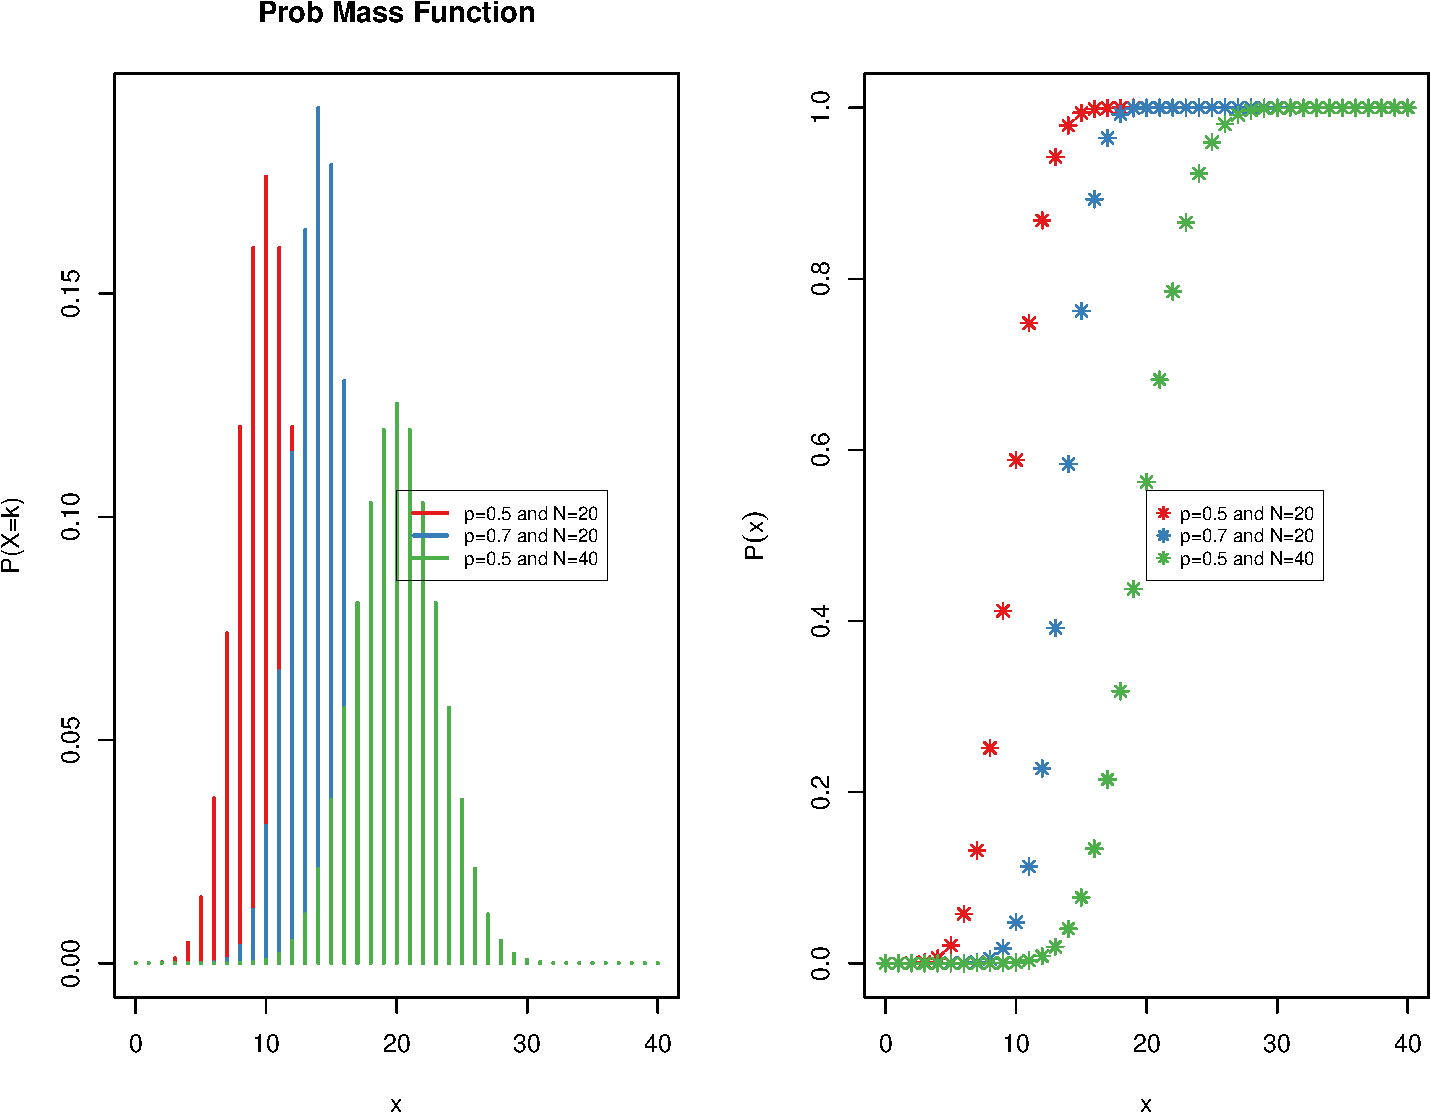
\includegraphics{tema4_files/figure-latex/unnamed-chunk-1-1.pdf}

con \emph{media} \(np\) y \emph{varianza} \(np(1-p)\).

\textbf{Pregunta:}

Supongamos que en un examen de matemáticas hay 12 preguntas de respuesta
múltiple. Cada una de las pregunras tiene 5 posibles respuestas de las
cuáles tan sólo una de ellas es correcta.

\begin{itemize}
\tightlist
\item
  ¿Cuál es la probabilidad de obtener 4 o menos respuestas correctas si
  un estudiante contesta al azar?
\end{itemize}

\begin{itemize}
\tightlist
\item
  ¿Cuál es la probabilidad de que el alumno tenga 2 ó 3 respuestas
  correctas?
\end{itemize}

\textbf{Pregunta:}

Supongamos que la empresa \emph{A} produce el producto \emph{B} con una
probabilidad de 0,005 de productos defectuosos. Supón que el prodcuto
\emph{B} se distribuye en lotes de 25 items. ¿Cuál es la probabilidad de
que un lote seleccionado al azar tenga exactamente 1 producto
defectuoso? ¿Cuál es la probabilidad de que un lote seleccionado al azar
no tenga más de un item defectuoso?

\textbf{Soluciones \href{IntroSM_sol.html}{aquí}}

\subsection{\texorpdfstring{Distribución de Poisson
\(Pois(\lambda)\)}{Distribución de Poisson Pois(\textbackslash{}lambda)}}\label{distribucion-de-poisson-poislambda}

La distribución de Poisson hace referencia a la modelización de
situaciones en las que nos interesa determinar el número de hechos de
cierto tipo que se pueden producir en un intervalo de tiempo o de
espacio. Si el parámetro \(\lambda\) es la media de sucesos por
intervalo, la probabilidad de tener \(k\) sucesos en el intervalo, se
define como la función de probabilidad de masa:

\[
\mbox{Pr}(\mbox{$k$ sucesos en el intervalo}) = \frac{\lambda^k e^{-\lambda}}{k!}
\]

La \textbf{función de densidad acumulada} es \[
P(X\leq x ~|~\lambda ) = \frac{e^{-\lambda} \lambda ^x}{x!}\quad \mbox{for $x=0,1,2,...$}
\]

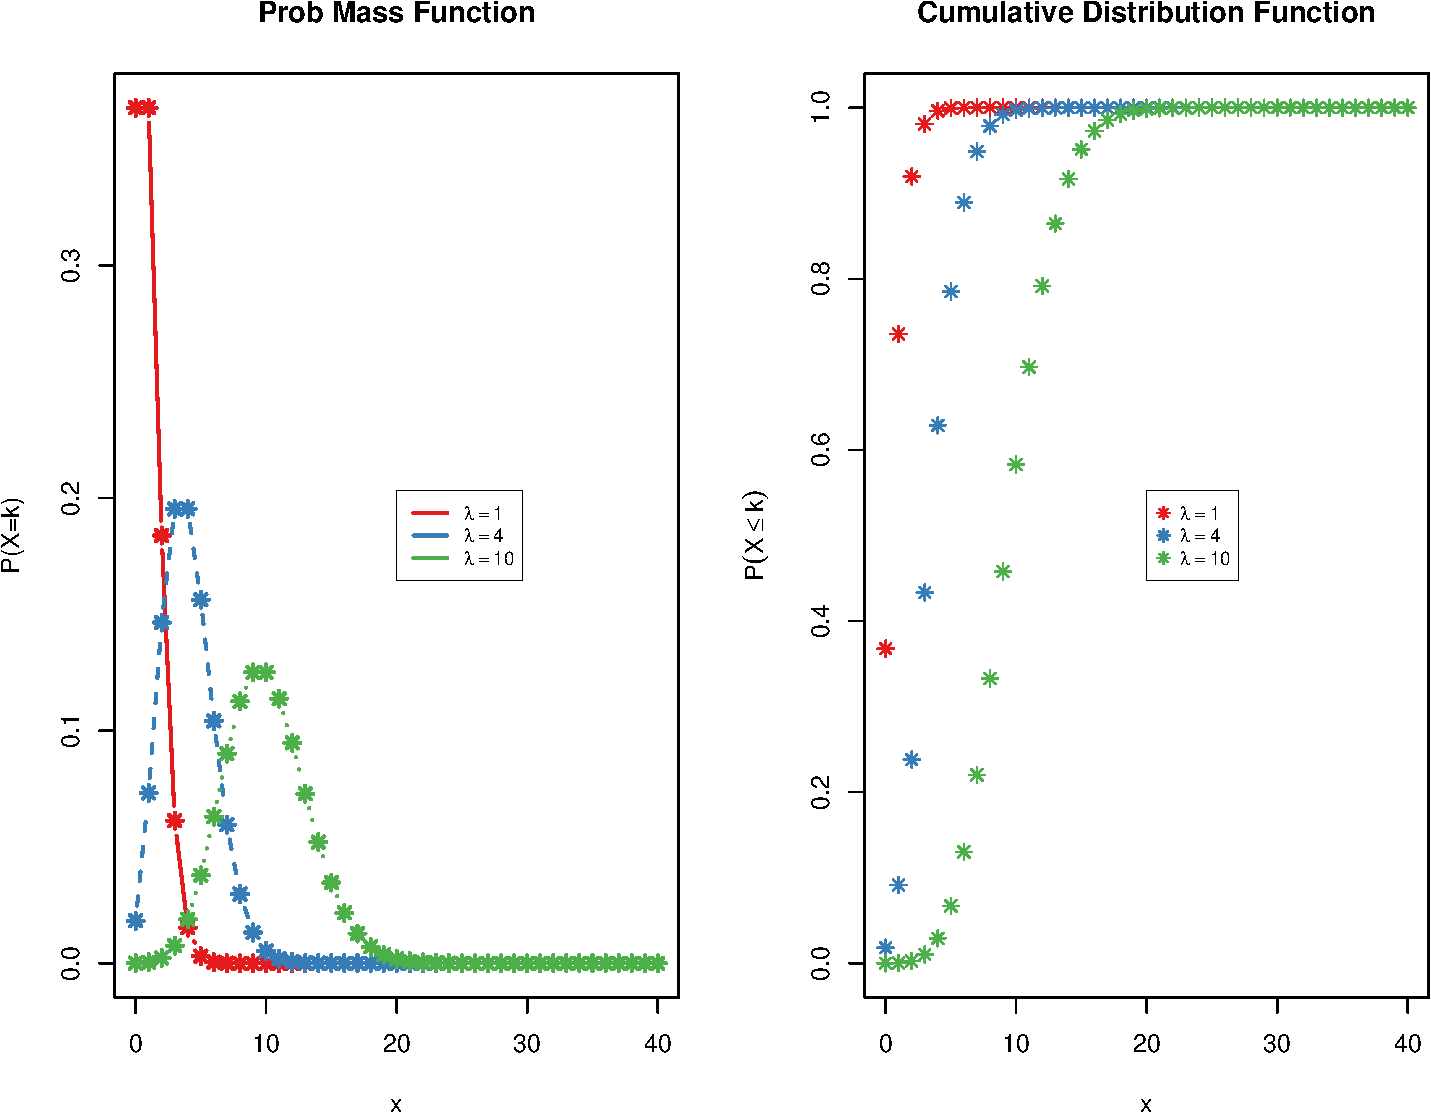
\includegraphics{tema4_files/figure-latex/unnamed-chunk-6-1.pdf}

\textbf{Pregunta:}

Supongamos que el número de insectos en una plantación de un metro
cuadrado, viene dada por una distribución de Poisson de media
\(\lambda= 10\). Calcula la probabilidad de encontrar exactamente \(12\)
insectos en una parcela de 1 \(m^2\).

\begin{verbatim}
## [1] 0.09478033
\end{verbatim}

\textbf{Pregunta:} Si hay 12 coches cruzando un puente por minuto en
media. Calcula la probabilidad de encontrar 17 ó más coches cruzando el
puente en un minuto cualquiera.

\textbf{Soluciones \href{IntroSM_sol.html}{aquí}}

\subsection{Aproximación de la Binomial y la
Poisson}\label{aproximacion-de-la-binomial-y-la-poisson}

\textbf{Ejemplo:}

El 5\% de las bombillas de un árbol de navidad manufacturado por una
compañia son defectuosas. El gerente del departamento de Control de
calidad de la empresa está preocupado y ha seleccionado 100 bombillas de
la cadena de montaje. Sea \(X\) el número de bombillas defectuosas.
¿Cuál es la probabilidad de que la muestra de 100 bombillas tenga a lo
sumo 3 bombillas defectuosas?

\begin{Shaded}
\begin{Highlighting}[]
\NormalTok{p =}\StringTok{ }\FloatTok{0.05}
\NormalTok{k =}\StringTok{ }\DecValTok{3}
\NormalTok{n =}\StringTok{ }\DecValTok{100}
\KeywordTok{pbinom}\NormalTok{(k,}\DataTypeTok{size=}\NormalTok{n,}\DataTypeTok{prob=}\NormalTok{p)}
\end{Highlighting}
\end{Shaded}

\begin{verbatim}
## [1] 0.2578387
\end{verbatim}

Se puede demostrar que la distribución Binomial se puede aproximar
mediante la distribución de Poisson cuando \(n\) es grande. Mediante la
distribución de Poisson, la media es \(\lambda = np\)

\begin{Shaded}
\begin{Highlighting}[]
\NormalTok{lambda <-}\StringTok{ }\NormalTok{n*p}
\KeywordTok{sum}\NormalTok{(}\KeywordTok{dpois}\NormalTok{(}\DecValTok{0}\NormalTok{:}\DecValTok{3}\NormalTok{,lambda))}
\end{Highlighting}
\end{Shaded}

\begin{verbatim}
## [1] 0.2650259
\end{verbatim}

Esta aproximación es válida con \(n\) grande y \(p\) pequeño. En
general, con \(n \geq 20\) y \(p\leq0.05\), o bien cuando \(n\geq 100\)
y \(p\leq 0.10\).

\subsection{\texorpdfstring{Distribucion exponencial
\(Exp(\lambda)\)}{Distribucion exponencial Exp(\textbackslash{}lambda)}}\label{distribucion-exponencial-explambda}

La distribución Exponencial mide la probabilidad de que una variable
aleatoria que describe el tiempo entre eventos de un proceso de Poisson,
es decir un proceso que ocurre de manera contínua e independiente a una
tasa constante. Es un caso particular de la distribución Gamma y el
análogo contínua de la distribución geométrica y tiene la propiedad de
falta de memoria.

La funcion de densidad de probabilidad es \[
f(x;\lambda) =  \lambda \exp(-\lambda x)
\]

donde \(\lambda>0\) es la tasa del evento (también conocido tasa de
llegadas, tasa de transición etc \ldots{}). Un variable aleatoria
Exponencial: \(x \in [0,\infty)\)
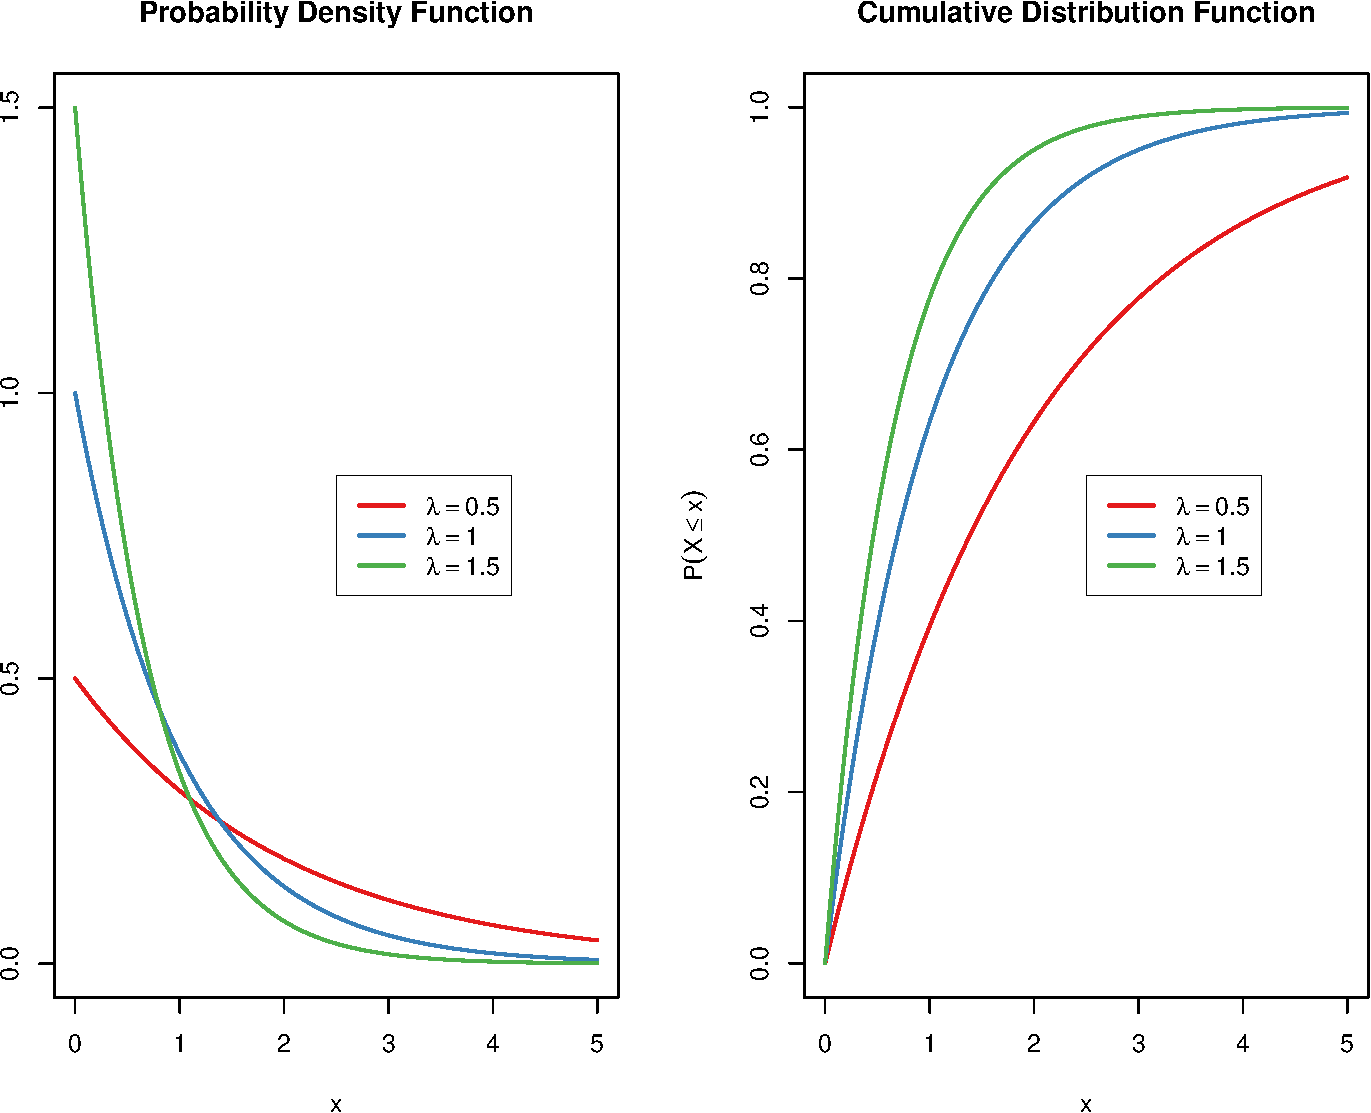
\includegraphics{tema4_files/figure-latex/unnamed-chunk-10-1.pdf}

La función de distribución acumulada es \[
F(x) = \mbox{Pr}(X\leq x) = 
  \left\{
    \begin{array}{lcc}
      1- e^{-\lambda x} & & x\geq 0 \\
      0                 & & x < 0
    \end{array}
  \right.
\]

La media \(\mathbb{E}(X) = 1/\lambda\), y
\(\mathbb{V}ar(X) = 1/\lambda^2\).

\textbf{Pregunta:} Supongamos que la cantidad de tiempo que los clientes
de un banco pasan en él se distribuye como una exponencial con media 10
minutos, por tanto \(\lambda=1/10\).

\begin{itemize}
\tightlist
\item
  ¿Cuál es la probabilidad de que un cliente pase más de 15 minutos en
  el banco?
\item
  ¿Cuál es la probabilidad de que un cliente pase más de 15 minutos en
  el banco dado que sigue en el banco después de 10 minutos?
\end{itemize}

\textbf{Soluciones \href{IntroSM_sol.html}{aquí}}

\subsection{\texorpdfstring{Distribución Normal
\(\mathcal{N}(\mu,\sigma^2)\)}{Distribución Normal \textbackslash{}mathcal\{N\}(\textbackslash{}mu,\textbackslash{}sigma\^{}2)}}\label{distribucion-normal-mathcalnmusigma2}

La función de densidad es

\[
f(x | \mu,\sigma^2) = \frac{1}{\sqrt{2\sigma^2\pi}} e ^{-\frac{(x-\mu)^2}{2\sigma^2}},
\] donde

\begin{itemize}
\tightlist
\item
  \(\mu\) es la media (tambien mediana y moda).
\item
  \(\sigma\) es la desviación estándar (\(\sigma>0\)).
\item
  \(\sigma^2\) la varianza.
\end{itemize}

El proceso de estandarización de la distribución Normal, consiste en
transformar una variable \(N(\mu,\sigma)\) en \(N(0,1)\), i.e. \[
Z = \frac{X-\mu}{\sigma} \sim N(0,1)
\]

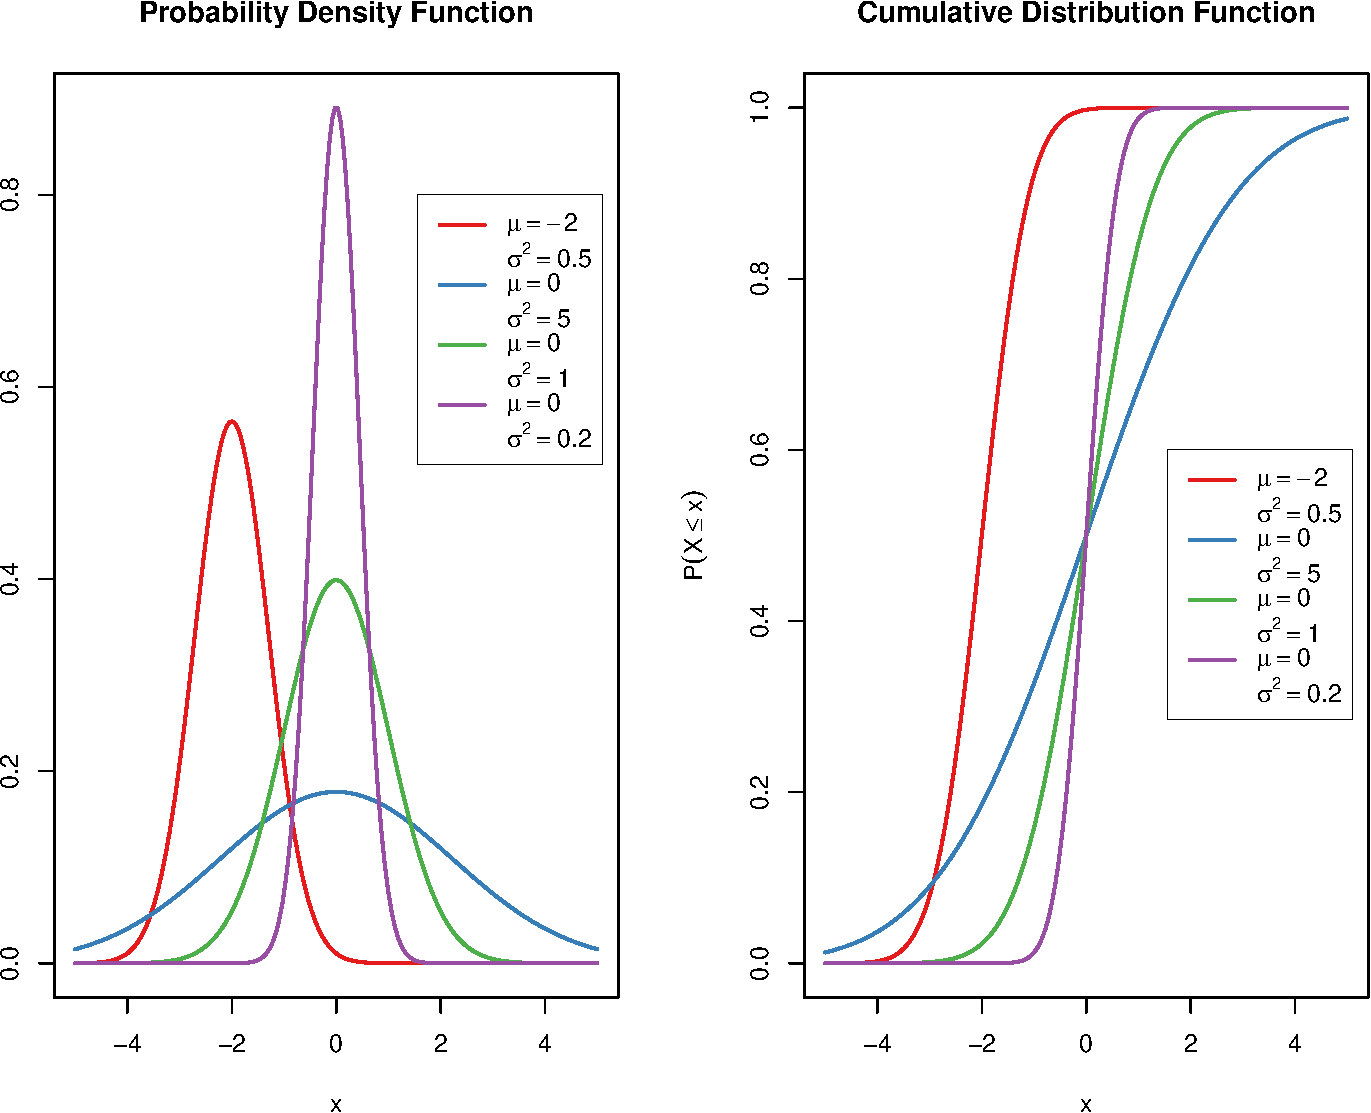
\includegraphics{tema4_files/figure-latex/unnamed-chunk-11-1.pdf}

\textbf{Pregunta:}

Sea \(X\) una variable aleatoria distribuida como una Normal con media
\(\mu = 30\) y desviación estandard \(\sigma = 4\). Calcula

\begin{enumerate}
\def\labelenumi{\alph{enumi})}
\item
  \(P(x<40)\)
\item
  \(P(x>21)\)
\item
  \(P(30<x<35)\)
\end{enumerate}

\textbf{Pregunta:}

El acceso a una Universdad viene dado por un examen a nivel Nacional.
Las puntuaciones de este examen se distribuyen mediante una distribución
Normal con media 500 y desviación estandard de 100. Tomás quiere ser
admitido a esta universidad y sabe que debe obtener una nota media
superior al 70\% de los estudiantes que hicieron el examen. Tomás sacó
una nota de 585. ¿Será admitido?

\textbf{Soluciones \href{IntroSM_sol.html}{aquí}}

\end{document}